\documentclass[twoside]{book}

% Packages required by doxygen
\usepackage{fixltx2e}
\usepackage{calc}
\usepackage{doxygen}
\usepackage[export]{adjustbox} % also loads graphicx
\usepackage{graphicx}
\usepackage[utf8]{inputenc}
\usepackage{makeidx}
\usepackage{multicol}
\usepackage{multirow}
\PassOptionsToPackage{warn}{textcomp}
\usepackage{textcomp}
\usepackage[nointegrals]{wasysym}
\usepackage[table]{xcolor}

% Font selection
\usepackage[T1]{fontenc}
\usepackage[scaled=.90]{helvet}
\usepackage{courier}
\usepackage{amssymb}
\usepackage{sectsty}
\renewcommand{\familydefault}{\sfdefault}
\allsectionsfont{%
  \fontseries{bc}\selectfont%
  \color{darkgray}%
}
\renewcommand{\DoxyLabelFont}{%
  \fontseries{bc}\selectfont%
  \color{darkgray}%
}
\newcommand{\+}{\discretionary{\mbox{\scriptsize$\hookleftarrow$}}{}{}}

% Page & text layout
\usepackage{geometry}
\geometry{%
  a4paper,%
  top=2.5cm,%
  bottom=2.5cm,%
  left=2.5cm,%
  right=2.5cm%
}
\tolerance=750
\hfuzz=15pt
\hbadness=750
\setlength{\emergencystretch}{15pt}
\setlength{\parindent}{0cm}
\setlength{\parskip}{0.2cm}
\makeatletter
\renewcommand{\paragraph}{%
  \@startsection{paragraph}{4}{0ex}{-1.0ex}{1.0ex}{%
    \normalfont\normalsize\bfseries\SS@parafont%
  }%
}
\renewcommand{\subparagraph}{%
  \@startsection{subparagraph}{5}{0ex}{-1.0ex}{1.0ex}{%
    \normalfont\normalsize\bfseries\SS@subparafont%
  }%
}
\makeatother

% Headers & footers
\usepackage{fancyhdr}
\pagestyle{fancyplain}
\fancyhead[LE]{\fancyplain{}{\bfseries\thepage}}
\fancyhead[CE]{\fancyplain{}{}}
\fancyhead[RE]{\fancyplain{}{\bfseries\leftmark}}
\fancyhead[LO]{\fancyplain{}{\bfseries\rightmark}}
\fancyhead[CO]{\fancyplain{}{}}
\fancyhead[RO]{\fancyplain{}{\bfseries\thepage}}
\fancyfoot[LE]{\fancyplain{}{}}
\fancyfoot[CE]{\fancyplain{}{}}
\fancyfoot[RE]{\fancyplain{}{\bfseries\scriptsize Generated on Thu Dec 10 2015 18\+:34\+:48 for Grappa R\+D\+D by Doxygen }}
\fancyfoot[LO]{\fancyplain{}{\bfseries\scriptsize Generated on Thu Dec 10 2015 18\+:34\+:48 for Grappa R\+D\+D by Doxygen }}
\fancyfoot[CO]{\fancyplain{}{}}
\fancyfoot[RO]{\fancyplain{}{}}
\renewcommand{\footrulewidth}{0.4pt}
\renewcommand{\chaptermark}[1]{%
  \markboth{#1}{}%
}
\renewcommand{\sectionmark}[1]{%
  \markright{\thesection\ #1}%
}

% Indices & bibliography
\usepackage{natbib}
\usepackage[titles]{tocloft}
\setcounter{tocdepth}{3}
\setcounter{secnumdepth}{5}
\makeindex

% Hyperlinks (required, but should be loaded last)
\usepackage{ifpdf}
\ifpdf
  \usepackage[pdftex,pagebackref=true]{hyperref}
\else
  \usepackage[ps2pdf,pagebackref=true]{hyperref}
\fi
\hypersetup{%
  colorlinks=true,%
  linkcolor=blue,%
  citecolor=blue,%
  unicode%
}

% Custom commands
\newcommand{\clearemptydoublepage}{%
  \newpage{\pagestyle{empty}\cleardoublepage}%
}


%===== C O N T E N T S =====

\begin{document}

% Titlepage & ToC
\hypersetup{pageanchor=false,
             bookmarks=true,
             bookmarksnumbered=true,
             pdfencoding=unicode
            }
\pagenumbering{roman}
\begin{titlepage}
\vspace*{7cm}
\begin{center}%
{\Large Grappa R\+D\+D }\\
\vspace*{1cm}
{\large Generated by Doxygen 1.8.10}\\
\vspace*{0.5cm}
{\small Thu Dec 10 2015 18:34:48}\\
\end{center}
\end{titlepage}
\clearemptydoublepage
\tableofcontents
\clearemptydoublepage
\pagenumbering{arabic}
\hypersetup{pageanchor=true}

%--- Begin generated contents ---
\chapter{Grappa\+R\+D\+D}
\label{md__r_e_a_d_m_e}
\hypertarget{md__r_e_a_d_m_e}{}
Implementation of Resilient Distributed Datasets from Apache Spark with distributed share memory using Grappa 
\chapter{Hierarchical Index}
\section{Class Hierarchy}
This inheritance list is sorted roughly, but not completely, alphabetically\+:\begin{DoxyCompactList}
\item \contentsline{section}{double\+\_\+container}{\pageref{structdouble__container}}{}
\item \contentsline{section}{Grappa\+Context}{\pageref{class_grappa_context}}{}
\item \contentsline{section}{int\+\_\+container}{\pageref{structint__container}}{}
\item \contentsline{section}{R\+D\+D$<$ A $>$}{\pageref{class_r_d_d}}{}
\begin{DoxyCompactList}
\item \contentsline{section}{Mapped\+R\+D\+D$<$ T, A $>$}{\pageref{class_mapped_r_d_d}}{}
\item \contentsline{section}{Parallel\+Collection\+R\+D\+D$<$ A $>$}{\pageref{class_parallel_collection_r_d_d}}{}
\item \contentsline{section}{Ranged\+R\+D\+D$<$ A $>$}{\pageref{class_ranged_r_d_d}}{}
\end{DoxyCompactList}
\item \contentsline{section}{R\+D\+D$<$ T $>$}{\pageref{class_r_d_d}}{}
\end{DoxyCompactList}

\chapter{Class Index}
\section{Class List}
Here are the classes, structs, unions and interfaces with brief descriptions\+:\begin{DoxyCompactList}
\item\contentsline{section}{\hyperlink{structdouble__container}{double\+\_\+container} }{\pageref{structdouble__container}}{}
\item\contentsline{section}{\hyperlink{class_grappa_context}{Grappa\+Context} }{\pageref{class_grappa_context}}{}
\item\contentsline{section}{\hyperlink{structint__container}{int\+\_\+container} }{\pageref{structint__container}}{}
\item\contentsline{section}{\hyperlink{class_mapped_r_d_d}{Mapped\+R\+D\+D$<$ T, A $>$} }{\pageref{class_mapped_r_d_d}}{}
\item\contentsline{section}{\hyperlink{class_parallel_collection_r_d_d}{Parallel\+Collection\+R\+D\+D$<$ A $>$} }{\pageref{class_parallel_collection_r_d_d}}{}
\item\contentsline{section}{\hyperlink{class_ranged_r_d_d}{Ranged\+R\+D\+D$<$ A $>$} }{\pageref{class_ranged_r_d_d}}{}
\item\contentsline{section}{\hyperlink{class_r_d_d}{R\+D\+D$<$ A $>$} }{\pageref{class_r_d_d}}{}
\end{DoxyCompactList}

\chapter{Class Documentation}
\hypertarget{structdouble__container}{}\section{double\+\_\+container Struct Reference}
\label{structdouble__container}\index{double\+\_\+container@{double\+\_\+container}}
\subsection*{Public Attributes}
\begin{DoxyCompactItemize}
\item 
\hypertarget{structdouble__container_a9fd1d983a0ea24d4728f04908c2f9d55}{}double {\bfseries a}\label{structdouble__container_a9fd1d983a0ea24d4728f04908c2f9d55}

\item 
\hypertarget{structdouble__container_af498e61611f93486e159bfd39403d968}{}double {\bfseries b}\label{structdouble__container_af498e61611f93486e159bfd39403d968}

\end{DoxyCompactItemize}


The documentation for this struct was generated from the following file\+:\begin{DoxyCompactItemize}
\item 
main.\+cpp\end{DoxyCompactItemize}

\hypertarget{class_grappa_context}{}\section{Grappa\+Context Class Reference}
\label{class_grappa_context}\index{Grappa\+Context@{Grappa\+Context}}
\subsection*{Public Member Functions}
\begin{DoxyCompactItemize}
\item 
\hypertarget{class_grappa_context_acc13cc44a53da592e1f7ce81f9a84b61}{}{\bfseries Grappa\+Context} (int argc, char $\ast$argv\mbox{[}$\,$\mbox{]})\label{class_grappa_context_acc13cc44a53da592e1f7ce81f9a84b61}

\item 
\hypertarget{class_grappa_context_aacb2d930729185106f8aa2ac222b79f3}{}void {\bfseries run} (void($\ast$fp)())\label{class_grappa_context_aacb2d930729185106f8aa2ac222b79f3}

\item 
\hypertarget{class_grappa_context_a5081d79c66a5c6b044e94687aa434d00}{}void {\bfseries stop} ()\label{class_grappa_context_a5081d79c66a5c6b044e94687aa434d00}

\end{DoxyCompactItemize}


The documentation for this class was generated from the following file\+:\begin{DoxyCompactItemize}
\item 
Grappa\+Context.\+hpp\end{DoxyCompactItemize}

\hypertarget{structint__container}{}\section{int\+\_\+container Struct Reference}
\label{structint__container}\index{int\+\_\+container@{int\+\_\+container}}
\subsection*{Public Attributes}
\begin{DoxyCompactItemize}
\item 
\hypertarget{structint__container_a8bc1b0e8ac42abc46d88004d7004e989}{}int64\+\_\+t {\bfseries a}\label{structint__container_a8bc1b0e8ac42abc46d88004d7004e989}

\item 
\hypertarget{structint__container_a31f640d6f13abb7044e85a811fd3d340}{}int64\+\_\+t {\bfseries b}\label{structint__container_a31f640d6f13abb7044e85a811fd3d340}

\end{DoxyCompactItemize}


The documentation for this struct was generated from the following file\+:\begin{DoxyCompactItemize}
\item 
main.\+cpp\end{DoxyCompactItemize}

\hypertarget{class_mapped_r_d_d}{}\section{Mapped\+R\+D\+D$<$ T, A $>$ Class Template Reference}
\label{class_mapped_r_d_d}\index{Mapped\+R\+D\+D$<$ T, A $>$@{Mapped\+R\+D\+D$<$ T, A $>$}}
Inheritance diagram for Mapped\+R\+D\+D$<$ T, A $>$\+:\begin{figure}[H]
\begin{center}
\leavevmode
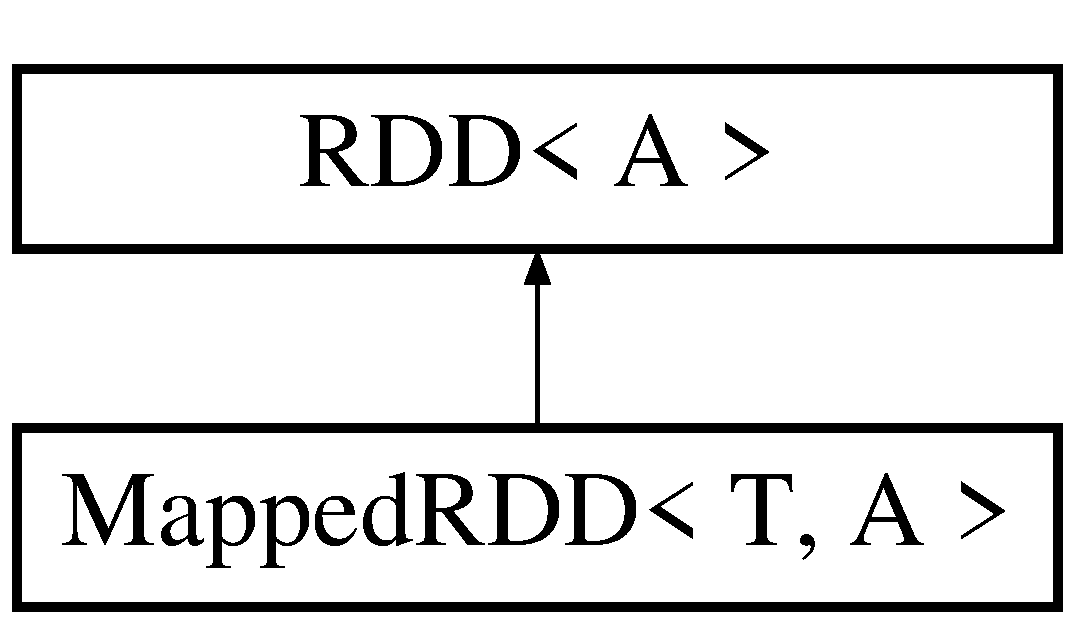
\includegraphics[height=2.000000cm]{class_mapped_r_d_d}
\end{center}
\end{figure}
\subsection*{Public Member Functions}
\begin{DoxyCompactItemize}
\item 
\hypertarget{class_mapped_r_d_d_a4926bf8d96b3aa0d7e8d2ce2ea3ae71c}{}{\bfseries Mapped\+R\+D\+D} (\hyperlink{class_r_d_d}{R\+D\+D}$<$ T $>$ $\ast$prev, std\+::function$<$ A(T)$>$ f)\label{class_mapped_r_d_d_a4926bf8d96b3aa0d7e8d2ce2ea3ae71c}

\item 
\hypertarget{class_mapped_r_d_d_a4f6d501824803f296effe1da1155cb62}{}Global\+Address$<$ A $>$ {\bfseries compute} ()\label{class_mapped_r_d_d_a4f6d501824803f296effe1da1155cb62}

\end{DoxyCompactItemize}
\subsection*{Public Attributes}
\begin{DoxyCompactItemize}
\item 
\hypertarget{class_mapped_r_d_d_a24c0005ebdadd20729034f12f5ea95fc}{}\hyperlink{class_r_d_d}{R\+D\+D}$<$ T $>$ $\ast$ {\bfseries prev}\label{class_mapped_r_d_d_a24c0005ebdadd20729034f12f5ea95fc}

\item 
\hypertarget{class_mapped_r_d_d_a0793f60e9e6a3d6433f207a7fd277fd2}{}std\+::function$<$ A(T)$>$ {\bfseries f}\label{class_mapped_r_d_d_a0793f60e9e6a3d6433f207a7fd277fd2}

\end{DoxyCompactItemize}
\subsection*{Additional Inherited Members}


The documentation for this class was generated from the following file\+:\begin{DoxyCompactItemize}
\item 
R\+D\+D.\+hpp\end{DoxyCompactItemize}

\hypertarget{class_parallel_collection_r_d_d}{}\section{Parallel\+Collection\+R\+D\+D$<$ A $>$ Class Template Reference}
\label{class_parallel_collection_r_d_d}\index{Parallel\+Collection\+R\+D\+D$<$ A $>$@{Parallel\+Collection\+R\+D\+D$<$ A $>$}}
Inheritance diagram for Parallel\+Collection\+R\+D\+D$<$ A $>$\+:\begin{figure}[H]
\begin{center}
\leavevmode
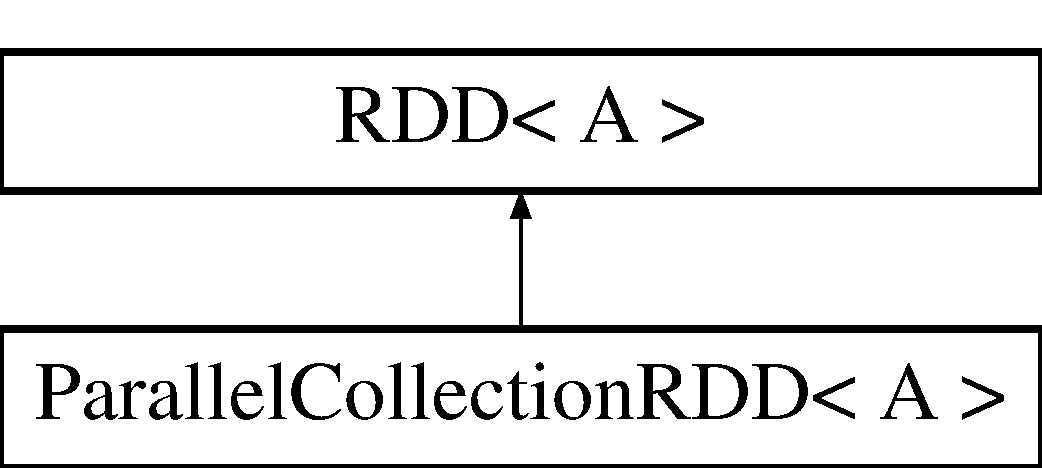
\includegraphics[height=2.000000cm]{class_parallel_collection_r_d_d}
\end{center}
\end{figure}
\subsection*{Public Member Functions}
\begin{DoxyCompactItemize}
\item 
\hypertarget{class_parallel_collection_r_d_d_ab0978f72535ee1744d26e785b66471ce}{}{\bfseries Parallel\+Collection\+R\+D\+D} (vector$<$ A $>$ sequence)\label{class_parallel_collection_r_d_d_ab0978f72535ee1744d26e785b66471ce}

\item 
\hypertarget{class_parallel_collection_r_d_d_ae68b0397be4483120fe2084fbb09f2b1}{}Global\+Address$<$ A $>$ {\bfseries compute} ()\label{class_parallel_collection_r_d_d_ae68b0397be4483120fe2084fbb09f2b1}

\end{DoxyCompactItemize}
\subsection*{Additional Inherited Members}


The documentation for this class was generated from the following file\+:\begin{DoxyCompactItemize}
\item 
R\+D\+D.\+hpp\end{DoxyCompactItemize}

\hypertarget{class_ranged_r_d_d}{}\section{Ranged\+R\+D\+D$<$ A $>$ Class Template Reference}
\label{class_ranged_r_d_d}\index{Ranged\+R\+D\+D$<$ A $>$@{Ranged\+R\+D\+D$<$ A $>$}}
Inheritance diagram for Ranged\+R\+D\+D$<$ A $>$\+:\begin{figure}[H]
\begin{center}
\leavevmode
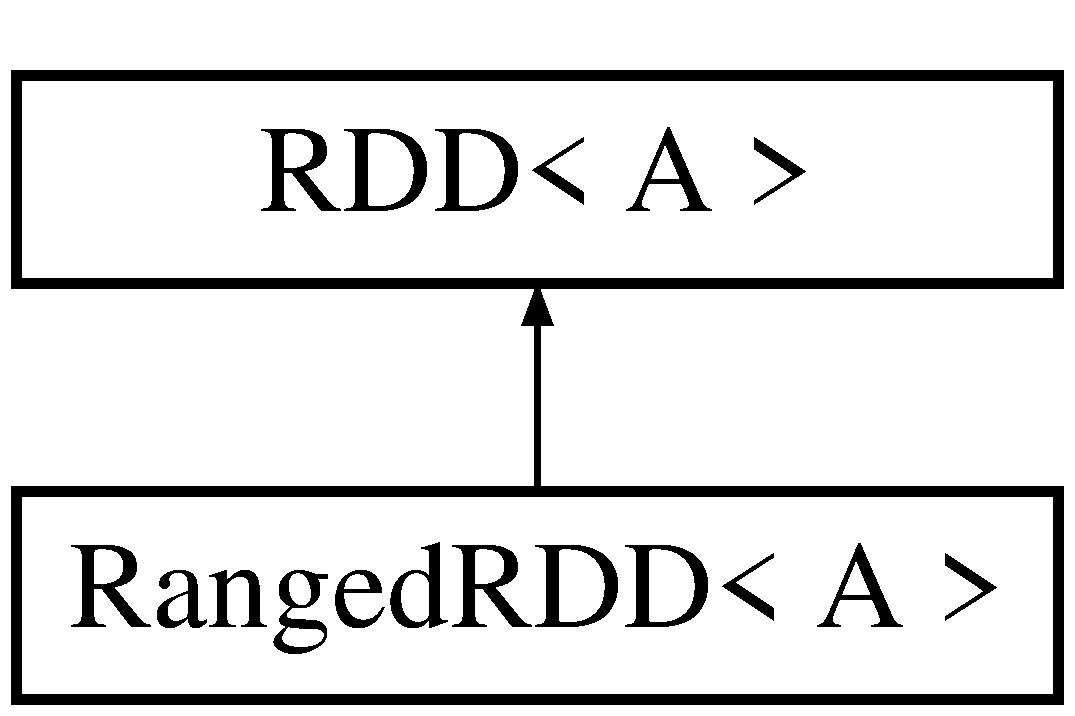
\includegraphics[height=2.000000cm]{class_ranged_r_d_d}
\end{center}
\end{figure}
\subsection*{Public Member Functions}
\begin{DoxyCompactItemize}
\item 
\hypertarget{class_ranged_r_d_d_ad6639a02411c8f03d2443e250720ec5a}{}{\bfseries Ranged\+R\+D\+D} (A start, A end)\label{class_ranged_r_d_d_ad6639a02411c8f03d2443e250720ec5a}

\item 
\hypertarget{class_ranged_r_d_d_a556bf430ea4bf9762b46fdaf3a23ac42}{}Global\+Address$<$ A $>$ {\bfseries compute} ()\label{class_ranged_r_d_d_a556bf430ea4bf9762b46fdaf3a23ac42}

\end{DoxyCompactItemize}
\subsection*{Additional Inherited Members}


The documentation for this class was generated from the following file\+:\begin{DoxyCompactItemize}
\item 
R\+D\+D.\+hpp\end{DoxyCompactItemize}

\hypertarget{class_r_d_d}{}\section{R\+D\+D$<$ A $>$ Class Template Reference}
\label{class_r_d_d}\index{R\+D\+D$<$ A $>$@{R\+D\+D$<$ A $>$}}
Inheritance diagram for R\+D\+D$<$ A $>$\+:\begin{figure}[H]
\begin{center}
\leavevmode
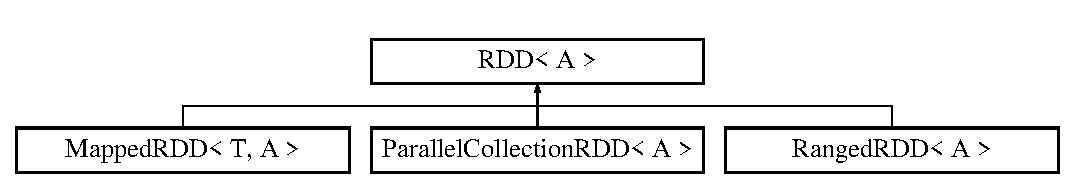
\includegraphics[height=2.000000cm]{class_r_d_d}
\end{center}
\end{figure}
\subsection*{Public Member Functions}
\begin{DoxyCompactItemize}
\item 
\hypertarget{class_r_d_d_adcb93ee8214e2be3dadd74da19bf3956}{}{\footnotesize template$<$typename Func $>$ }\\auto {\bfseries map} (Func f) -\/$>$ \hyperlink{class_r_d_d}{R\+D\+D}$<$ decltype(f(A()))$>$ $\ast$\label{class_r_d_d_adcb93ee8214e2be3dadd74da19bf3956}

\item 
auto \hyperlink{class_r_d_d_afb3f661ea1cc3aac6dbe66f764de1e43}{fold} (A init, A($\ast$f)(const A \&, const A \&)) -\/$>$ A
\item 
\hypertarget{class_r_d_d_a3e89daeddd050a5d6577e41f58b27b8c}{}A {\bfseries sum} ()\label{class_r_d_d_a3e89daeddd050a5d6577e41f58b27b8c}

\item 
\hypertarget{class_r_d_d_abbd3422e2760f4ca3af308cfb2606d50}{}A {\bfseries product} ()\label{class_r_d_d_abbd3422e2760f4ca3af308cfb2606d50}

\item 
\hypertarget{class_r_d_d_acd0b3de3863764e77ac9729a152f87c0}{}auto {\bfseries collect} () -\/$>$ vector$<$ A $>$\label{class_r_d_d_acd0b3de3863764e77ac9729a152f87c0}

\item 
\hypertarget{class_r_d_d_a3cee954e8f79a7066659ee4684fa7011}{}void {\bfseries print} ()\label{class_r_d_d_a3cee954e8f79a7066659ee4684fa7011}

\item 
\hypertarget{class_r_d_d_a7cbde0c28cf2ec9db04344e1e32e7217}{}virtual Global\+Address$<$ A $>$ {\bfseries compute} ()=0\label{class_r_d_d_a7cbde0c28cf2ec9db04344e1e32e7217}

\end{DoxyCompactItemize}
\subsection*{Static Public Member Functions}
\begin{DoxyCompactItemize}
\item 
\hypertarget{class_r_d_d_abf5c7a7da50a4b5ff2ebc382ed2a3720}{}static \hyperlink{class_ranged_r_d_d}{Ranged\+R\+D\+D}$<$ A $>$ $\ast$ {\bfseries range} (A start, A end)\label{class_r_d_d_abf5c7a7da50a4b5ff2ebc382ed2a3720}

\item 
\hypertarget{class_r_d_d_acfa2ab9edf80c598f917a42aa08f6b85}{}static \hyperlink{class_ranged_r_d_d}{Ranged\+R\+D\+D}$<$ A $>$ $\ast$ {\bfseries range} (A end)\label{class_r_d_d_acfa2ab9edf80c598f917a42aa08f6b85}

\end{DoxyCompactItemize}
\subsection*{Protected Attributes}
\begin{DoxyCompactItemize}
\item 
\hypertarget{class_r_d_d_ad6d07c0d1bc8894b8dc15ac80cf6f73b}{}int {\bfseries size}\label{class_r_d_d_ad6d07c0d1bc8894b8dc15ac80cf6f73b}

\item 
\hypertarget{class_r_d_d_ab77cd5f6dbfea70169ea3c91e227f589}{}Global\+Address$<$ A $>$ {\bfseries rdd\+\_\+address}\label{class_r_d_d_ab77cd5f6dbfea70169ea3c91e227f589}

\end{DoxyCompactItemize}
\subsection*{Friends}
\begin{DoxyCompactItemize}
\item 
\hypertarget{class_r_d_d_aa90384db8e0bab61dfec3a641938e7db}{}{\footnotesize template$<$typename T , typename U $>$ }\\class {\bfseries Mapped\+R\+D\+D}\label{class_r_d_d_aa90384db8e0bab61dfec3a641938e7db}

\end{DoxyCompactItemize}


\subsection{Member Function Documentation}
\hypertarget{class_r_d_d_afb3f661ea1cc3aac6dbe66f764de1e43}{}\index{R\+D\+D@{R\+D\+D}!fold@{fold}}
\index{fold@{fold}!R\+D\+D@{R\+D\+D}}
\subsubsection[{fold(\+A init, A($\ast$f)(const A \&, const A \&)) -\/$>$ A}]{\setlength{\rightskip}{0pt plus 5cm}template$<$typename A$>$ auto {\bf R\+D\+D}$<$ A $>$\+::fold (
\begin{DoxyParamCaption}
\item[{A}]{init, }
\item[{A($\ast$)(const A \&, const A \&)}]{f}
\end{DoxyParamCaption}
) -\/$>$ A \hspace{0.3cm}{\ttfamily [inline]}}\label{class_r_d_d_afb3f661ea1cc3aac6dbe66f764de1e43}
Folds the \hyperlink{class_r_d_d}{R\+D\+D} to a single value using f.


\begin{DoxyParams}{Parameters}
{\em init} & Initial vale for fold \\
\hline
{\em f} & Function which folds elements by (A, A) -\/$>$ A \\
\hline
\end{DoxyParams}
\begin{DoxyReturn}{Returns}
\hyperlink{class_r_d_d}{R\+D\+D} reduced using f 
\end{DoxyReturn}


The documentation for this class was generated from the following file\+:\begin{DoxyCompactItemize}
\item 
R\+D\+D.\+hpp\end{DoxyCompactItemize}

%--- End generated contents ---

% Index
\backmatter
\newpage
\phantomsection
\clearemptydoublepage
\addcontentsline{toc}{chapter}{Index}
\printindex

\end{document}
